\documentclass{article}

\usepackage{epsfig,graphics,psfrag,color,rotating}
\usepackage{amsmath,amsfonts,amssymb,bbm}

\textwidth=30cm

\sloppy


\begin{document}
\thispagestyle{empty}

\begin{figure}
%
\centerline{ 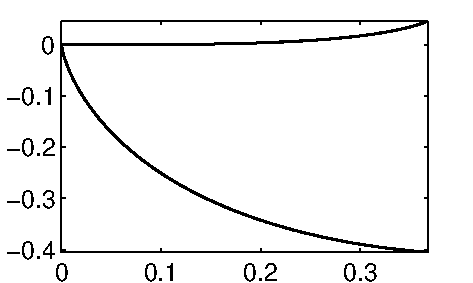
\includegraphics[width=5cm]{../EPS/Phi_Gamma_a2_p2} \hspace{2mm}
  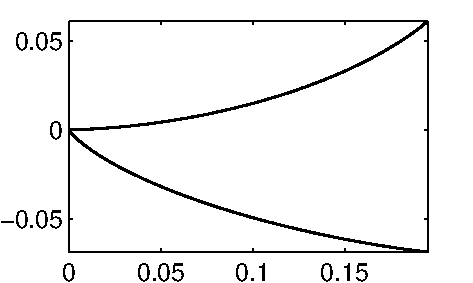
\includegraphics[width=5cm]{../EPS/Phi_Gamma_a5_p2}}
%
\begin{picture}(0,0)
\put(340,97){$\alpha = 2$}
\put(360,75){$\phi_0$}
\put(342,40){$\phi_{-1}$}
\put(350,3){$y$}
%
\put(495,97){$\alpha = 5$}
\put(520,75){$\phi_0$}
\put(520,33){$\phi_{-1}$}
\put(505,3){$y$}
\end{picture}
\end{figure}

\end{document}